\documentclass{article}

\usepackage{pandekten}
\usepackage{dashrule}

\makeatletter
\newcommand*{\shifttext}[1]{%
  \settowidth{\@tempdima}{#1}%
  \hspace{-\@tempdima}#1%
}
\newcommand{\plabel}[1]{%
\shifttext{\textbf{#1}\quad}%
}
\newcommand{\prule}{%
\begin{center}%
\hdashrule[0.5ex]{.99\linewidth}{1pt}{1pt 2.5pt}%
\end{center}%
}

\makeatother

\newcommand{\minusbaseline}{\abovedisplayskip=0pt\abovedisplayshortskip=0pt~\vspace*{-\baselineskip}}%

\setlength{\parindent}{0pt}

\title{Assignment 5}
\author{Ze Chen}

\begin{document}

\maketitle

\plabel{1 (a)}%
Under RWA, the equation becomes
\begin{align*}
    \dot{a}_1 &= i\Omega_{\mathrm{R}} e^{i\Delta \cdot t} a_2, \\
    \dot{a}_2 &= i\Omega_{\mathrm{R}} e^{-i\Delta \cdot t} a_1, \\
    a_1(0) &= 1,\quad a_2(0) = 0.
\end{align*}
The solution is given by
\begin{align*}
    a_1(t) &= \frac{e^{{i \Delta  t}/{2}} (2 \Omega  \cos (\Omega t )-i \Delta  \sin (\Omega t ))}{2 \Omega }, \\
    a_2(t) &= i \frac{\Omega_{\mathrm{R}}}{\Omega} e^{-i\Delta t / 2} \sin(\Omega t), \\
    \Omega &= \sqrt{\frac{\Delta^2}{4} + \Omega_{\mathrm{R}}^2}.
\end{align*}

\plabel{(b)}%
The plots are given for $\Omega = \Omega_{\mathrm{R}} \sqrt{1 + \alpha^2/4}$ where $\alpha = \qty{0, 0.1, 1, 10}$.
\begin{center}
    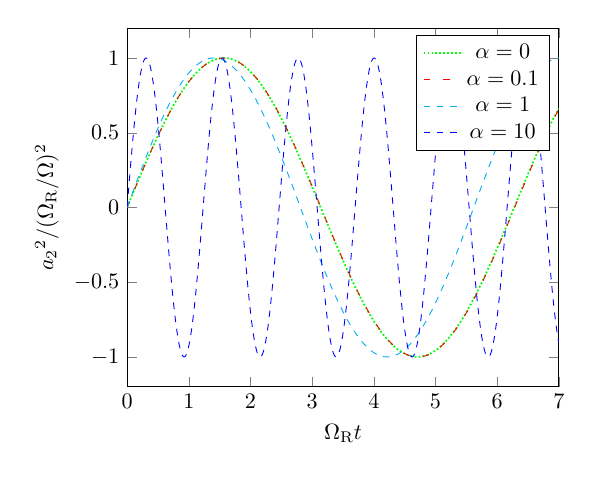
\begin{tikzpicture}[scale=0.8]
        \begin{axis}[xmin=0, xmax=7, samples=1000, xlabel=$\Omega_{\mathrm{R}}t$,ylabel=$\abs{a_2}^2/(\Omega_{\mathrm{R}}/\Omega)^2$]
          \addplot[densely dotted, thick, draw=green, domain=0:7] (x, {sin(x/pi*180*sqrt(1+0.1^2/4))});
          \addplot[loosely dashed, draw=red, domain=0:7] (x, {sin(x/pi*180)});
          \addplot[dashed, draw=cyan, domain=0:7] (x, {sin(x/pi*180*sqrt(1+1^2/4))});
          \addplot[dashed, draw=blue, domain=0:7] (x, {sin(x/pi*180*sqrt(1+10^2/4))});
          \legend{$\alpha=0$,$\alpha=0.1$,$\alpha=1$,$\alpha=10$}
        \end{axis}
    \end{tikzpicture}
\end{center}
Moving away from resonance increases the effective frequency.

\plabel{(c)}%
\begingroup\minusbaseline
\begin{center}
    \begin{tikzpicture}[scale=0.6]
        \begin{axis}[title={$\Omega_{\mathrm{R}}/\omega_{12}=0.1$},name=plot1,ylabel=$\abs{a_2}^2$]
            \addplot[-,red] table {data0.1.txt};
            \addlegendentry{Exact};
            \addplot[-,blue] table {dataA0.1.txt};
            \addlegendentry{RWA};
        \end{axis}
        \begin{axis}[title={$\Omega_{\mathrm{R}}/\omega_{12}=0.3$},name=plot2,at=(plot1.right of east),anchor=left of west]
            \addplot[-,red] table {data0.3.txt};
            \addlegendentry{Exact};
            \addplot[-,blue] table {dataA0.3.txt};
            \addlegendentry{RWA};
        \end{axis}
        \begin{axis}[title={$\Omega_{\mathrm{R}}/\omega_{12}=0.5$},name=plot3,at=(plot1.below south),anchor=above north,xlabel=$\omega_{12}t$,ylabel=$\abs{a_2}^2$]
            \addplot[-,red] table {data0.5.txt};
            \addlegendentry{Exact};
            \addplot[-,blue] table {dataA0.5.txt};
            \addlegendentry{RWA};
        \end{axis}
        \begin{axis}[title={$\Omega_{\mathrm{R}}/\omega_{12}=1$},name=plot4,at=(plot2.below south),anchor=above north,xlabel=$\omega_{12}t$]
            \addplot[-,red] table {data1.txt};
            \addlegendentry{Exact};
            \addplot[-,blue] table {dataA1.txt};
            \addlegendentry{RWA};
        \end{axis}
    \end{tikzpicture}
\end{center}
\endgroup

\plabel{(d)}%
\begingroup\minusbaseline
\begin{center}
    \begin{tikzpicture}[scale=0.6]
        \begin{axis}[title={$\Omega_{\mathrm{R}}/\omega_{12}=0.1$},name=plot1,ylabel=$\abs{\tilde{a}_2}$]
            \addplot[-,red] table {fdata0.1.txt};
            \addlegendentry{Exact};
            \addplot[-,blue] table {fdataA0.1.txt};
            \addlegendentry{RWA};
        \end{axis}
        \begin{axis}[title={$\Omega_{\mathrm{R}}/\omega_{12}=0.3$},name=plot2,at=(plot1.right of east),anchor=left of west]
            \addplot[-,red] table {fdata0.3.txt};
            \addlegendentry{Exact};
            \addplot[-,blue] table {fdataA0.3.txt};
            \addlegendentry{RWA};
        \end{axis}
        \begin{axis}[title={$\Omega_{\mathrm{R}}/\omega_{12}=0.5$},name=plot3,at=(plot1.below south),anchor=above north,xlabel=$\omega$,ylabel=$\abs{\tilde{a}_2}$]
            \addplot[-,red] table {fdata0.5.txt};
            \addlegendentry{Exact};
            \addplot[-,blue] table {fdataA0.5.txt};
            \addlegendentry{RWA};
        \end{axis}
        \begin{axis}[title={$\Omega_{\mathrm{R}}/\omega_{12}=1$},name=plot4,at=(plot2.below south),anchor=above north,xlabel=$\omega$]
            \addplot[-,red] table {fdata1.txt};
            \addlegendentry{Exact};
            \addplot[-,blue] table {fdataA1.txt};
            \addlegendentry{RWA};
        \end{axis}
    \end{tikzpicture}
\end{center}
\endgroup
There are three peaks since
\[ \dot{a}_1 \sim (1+e^{-2 i\omega t}) a_2 \sim (1 + e^{-2i\omega t}) \sin(\Omega t). \]
The peaks are $\Omega$ and $\Omega\pm 2\omega$.
As $\Omega$ goes large, the approximation for $a_2$ becomes inaccurate and the peaks shift from these values.

\prule

\plabel{2 (a)}%
\begingroup\minusbaseline
\begin{align*}
    E(t) &= E_0 \cos(\omega t), \\
    p^+(t) &= \mathcal{P}_{12} a^*_1(t) a_2(t) e^{-i\omega_{12}t}, \\
    d(t) &= \abs{a_2(t)}^2 - \abs{a_1(t)}^2.
\end{align*}
\endgroup
Therefore,
\begin{align*}
    \dot{p}^+(t) &= -i\omega_{12}p^+(t) - \frac{i\mathcal{P}_{12}^2}{\hbar} E(t) d(t), \\
    \dot{d}(t) &= \frac{2i}{\hbar} E(t)\qty[(p^+)^*(t) - p^+(t)].
\end{align*}
Adding the damping term yields
\begin{align*}
    \dot{p}^+(t) &= (-i\omega_{12} - \gamma_\perp)p^+(t) - \frac{i\mathcal{P}_{12}^2}{\hbar} E(t) d(t), \\
    \dot{d}(t) &= -\gamma_\parallel(1+d(t)) + \frac{2i}{\hbar} E(t)\qty[(p^+)^*(t) - p^+(t)].
\end{align*}

\plabel{(b)}%
\begingroup\minusbaseline
\begin{align*}
    \dot{\tilde{p}}^+(t) &= (-i \omega_{12} + i\omega - \gamma_\perp) \tilde{p}^+ - \frac{i \mathcal{P}_{12}^2}{\hbar} E(t) d(t) e^{i\omega t}, \\
    \dot{d}(t) &= -\gamma_\parallel (1+d(t)) + \frac{2i}{\hbar} E(t) \qty[(\tilde{p}^+)^*(t) e^{i\omega t} - \tilde{p}^+(t) e^{-i\omega t}].
\end{align*}
\endgroup
With RWA, $E(t)e^{i\omega t} = E_0/2$ and $E(t) \qty[(\tilde{p}^+)^*(t) e^{i\omega t} - \tilde{p}^+(t) e^{-i\omega t}] = E_0/2\cdot \qty[(\tilde{p}^+)^*(t) - \tilde{p}^+(t)]$, and therefore
\begin{align*}
    \dot{\tilde{p}}^+(t) &= (-i (\omega_{12} - \omega) - \gamma_\perp) \tilde{p}^+ - \frac{i \mathcal{P}_{12}^2}{2 \hbar} E_0 d(t), \\
    \dot{d}(t) &= -\gamma_\parallel (1+d(t)) + \frac{i}{\hbar} E_0 \qty[(\tilde{p}^+)^*(t)  - \tilde{p}^+(t)].
\end{align*}

\plabel{(c)}%
Setting LHS to zero we find
\begin{align*}
    d &= -\qty(1 + \frac{E_0^2 \mathcal{P}_{12}^2 \gamma_\perp}{\hbar^2 \gamma_\parallel (\gamma^2_\perp + (\omega-\omega_{12})^2)})^{-1}, \\
    \tilde{p}^+ &= -\frac{\mathcal{P}_{12}^2 E_0}{2\hbar((\omega_{12} - \omega) - i\gamma_\perp)} d.
\end{align*}

\plabel{(d)}%
At resonance,
\begin{align*}
    \dv{}{\gamma_{\mathrm{sp}}t} \tilde{p}^+ &= -\tilde{p}^+ - i\frac{\Omega_{\mathrm{R}}}{\gamma_{\mathrm{sp}}} d, \\
    \dv{}{\gamma_{\mathrm{sp}}t} d &= -2(1+d) + 2i \frac{\Omega_{\mathrm{R}}}{\gamma_{\mathrm{sp}}} \qty[(\tilde{p}^+)^* - \tilde{p}^+].
\end{align*}
The plots of solutions are given below.
\pgfplotsset{
    compat=newest,
    scaled y ticks=false,
    yticklabel style={
        /pgf/number format/fixed,
        /pgf/number format/precision=5
    },
}
\begin{center}
    \begin{tikzpicture}[scale=0.7]
        \begin{axis}[title={$\Omega_{\mathrm{R}}/\gamma_{\mathrm{sp}}=0.01$},name=plot1,ylabel=$d$,xlabel={$\gamma_{\mathrm{sp}} t$}]
            \addplot[-,red] table {ddata0.01.txt};
            \addlegendentry{$d$};
        \end{axis}
        \begin{axis}[title={$\Omega_{\mathrm{R}}/\gamma_{\mathrm{sp}}=0.01$},name=plot2,at=(plot1.right of east),anchor=left of west,ylabel=$p$,xlabel={$\gamma_{\mathrm{sp}} t$}]
            \addplot[-,red] table {rpdata0.01.txt};
            \addlegendentry{$\Re p$};
            \addplot[-,blue] table {ipdata0.01.txt};
            \addlegendentry{$\Im p$};
        \end{axis}
    \end{tikzpicture}
\end{center}
\begin{center}
    \begin{tikzpicture}[scale=0.7]
        \begin{axis}[title={$\Omega_{\mathrm{R}}/\gamma_{\mathrm{sp}}=0.1$},name=plot1,ylabel=$d$,xlabel={$\gamma_{\mathrm{sp}} t$}]
            \addplot[-,red] table {ddata0.1.txt};
            \addlegendentry{$d$};
        \end{axis}
        \begin{axis}[title={$\Omega_{\mathrm{R}}/\gamma_{\mathrm{sp}}=0.1$},name=plot2,at=(plot1.right of east),anchor=left of west,ylabel=$p$,xlabel={$\gamma_{\mathrm{sp}} t$}]
            \addplot[-,red] table {rpdata0.1.txt};
            \addlegendentry{$\Re p$};
            \addplot[-,blue] table {ipdata0.1.txt};
            \addlegendentry{$\Im p$};
        \end{axis}
    \end{tikzpicture}
\end{center}
\begin{center}
    \begin{tikzpicture}[scale=0.7]
        \begin{axis}[title={$\Omega_{\mathrm{R}}/\gamma_{\mathrm{sp}}=1$},name=plot1,ylabel=$d$,xlabel={$\gamma_{\mathrm{sp}} t$}]
            \addplot[-,red] table {ddata1.txt};
            \addlegendentry{$d$};
        \end{axis}
        \begin{axis}[title={$\Omega_{\mathrm{R}}/\gamma_{\mathrm{sp}}=1$},name=plot2,at=(plot1.right of east),anchor=left of west,ylabel=$p$,xlabel={$\gamma_{\mathrm{sp}} t$}]
            \addplot[-,red] table {rpdata1.txt};
            \addlegendentry{$\Re p$};
            \addplot[-,blue] table {ipdata1.txt};
            \addlegendentry{$\Im p$};
        \end{axis}
    \end{tikzpicture}
\end{center}
\begin{center}
    \begin{tikzpicture}[scale=0.7]
        \begin{axis}[title={$\Omega_{\mathrm{R}}/\gamma_{\mathrm{sp}}=10$},name=plot1,ylabel=$d$,xlabel={$\gamma_{\mathrm{sp}} t$}]
            \addplot[-,red] table {ddata10.txt};
            \addlegendentry{$d$};
        \end{axis}
        \begin{axis}[title={$\Omega_{\mathrm{R}}/\gamma_{\mathrm{sp}}=10$},name=plot2,at=(plot1.right of east),anchor=left of west,ylabel=$p$,xlabel={$\gamma_{\mathrm{sp}} t$}]
            \addplot[-,red] table {rpdata10.txt};
            \addlegendentry{$\Re p$};
            \addplot[-,blue] table {ipdata10.txt};
            \addlegendentry{$\Im p$};
        \end{axis}
    \end{tikzpicture}
\end{center}
Positive inversion occurs at $\Omega_{\mathrm{R}}/\gamma_{\mathrm{sp}} > \num{1.532}$.
For $\gamma_{\mathrm{sp}} \rightarrow 0$, inversion oscillates.
\begin{center}
    \begin{tikzpicture}[scale=0.7]
        \begin{axis}[title={$\Omega_{\mathrm{R}}/\gamma_{\mathrm{sp}}=1.532$},name=plot1,ylabel=$d$,xlabel={$\gamma_{\mathrm{sp}} t$}]
            \addplot[-,red] table {ddata1.532.txt};
            \addlegendentry{$d$};
        \end{axis}
        \begin{axis}[title={$\Omega_{\mathrm{R}}/\gamma_{\mathrm{sp}}=10^3$},name=plot2,at=(plot1.right of east),anchor=left of west,ylabel=$d$,xlabel={$\gamma_{\mathrm{sp}} t$}]
            \addplot[-,red] table {ddata1000.txt};
            \addlegendentry{$d$};
        \end{axis}
    \end{tikzpicture}
\end{center}

% \bibliographystyle{plain}
% \bibliography{main}

\end{document}
